% ============================================================
%  Chapter 3 – Applying Evolution to Vehicle Routing Problems
%  Nature-Inspired Optimisation for Delivery Problems (2022)
%  Self-contained Beamer slides — reader-friendly format
% ============================================================
\documentclass[aspectratio=169,10pt]{beamer}

\usetheme{Madrid}
\usecolortheme{seahorse}
\setbeamertemplate{footline}[frame number]
\setbeamertemplate{navigation symbols}{}

% ── packages ─────────────────────────────────────────────────
\usepackage[utf8]{inputenc}
\usepackage[T1]{fontenc}
\usepackage{graphicx}
\usepackage{amsmath,amssymb}
\usepackage{booktabs}
\usepackage{listings}
\usepackage{xcolor}
\usepackage{microtype}
\usepackage{array}
\usepackage{colortbl}
\usepackage{tikz}
\usetikzlibrary{shapes.geometric,arrows.meta,positioning,fit,backgrounds}

\graphicspath{{figures/}}

% ── listings style ────────────────────────────────────────────
\lstdefinestyle{javastyle}{
  language=Java,
  basicstyle=\ttfamily\scriptsize,
  numbers=left,
  numberstyle=\tiny\color{gray},
  frame=single,
  backgroundcolor=\color{gray!7},
  keywordstyle=\color{blue!70!black}\bfseries,
  commentstyle=\color{green!50!black}\itshape,
  stringstyle=\color{red!60!black},
  breaklines=true,
  showstringspaces=false,
  tabsize=2,
  captionpos=b,
}

\lstdefinestyle{pythonstyle}{
  language=Python,
  basicstyle=\ttfamily\scriptsize,
  numbers=left,
  numberstyle=\tiny\color{gray},
  frame=single,
  backgroundcolor=\color{gray!7},
  keywordstyle=\color{blue!70!black}\bfseries,
  commentstyle=\color{green!50!black}\itshape,
  stringstyle=\color{red!60!black},
  breaklines=true,
  showstringspaces=false,
  tabsize=2,
  captionpos=b,
}

% ── title metadata ────────────────────────────────────────────
\title[Ch.3 Evolutionary VRP]{Chapter 3: Applying Evolution\\to Vehicle Routing Problems}
\subtitle{Nature-Inspired Optimisation for Delivery Problems (2022)}
\author{Lecture Notes}
\date{2026}

% ============================================================
\begin{document}

\begin{frame}
  \titlepage
\end{frame}

% ── table of contents ────────────────────────────────────────
\begin{frame}{Chapter Outline}
  \tableofcontents
\end{frame}

% ============================================================
\section{3.1 Evolutionary Computation}
% ============================================================

\begin{frame}[allowframebreaks]{3.1 Evolutionary Computation — The Big Idea}

  \textbf{Where does the idea come from?}
  Darwin's \emph{On the Origin of Species} (1859) proposed that species improve over generations
  through natural selection: individuals that are better adapted to their environment are more
  likely to survive and reproduce, passing their favourable traits to offspring.
  Evolutionary Computation borrows this mechanism and applies it to mathematical optimisation.

  \medskip
  \begin{block}{Core analogy}
    \begin{tabular}{ll}
      \toprule
      \textbf{Biology}        & \textbf{Optimisation}              \\
      \midrule
      Individual organism     & A candidate solution               \\
      Genome (DNA sequence)   & Encoded representation of a solution \\
      Fitness (survival rate) & Objective value (e.g.\ total distance) \\
      Population              & Set of candidate solutions         \\
      Reproduction            & Creating new solutions             \\
      Mutation                & Small random changes to a solution \\
      Crossover               & Combining parts of two solutions   \\
      Natural selection       & Preferring better solutions        \\
      \bottomrule
    \end{tabular}
  \end{block}

  \framebreak

  \textbf{The fitness landscape — a mental model.}
  Imagine every possible solution laid out on a map.
  The height of the map at any point represents the fitness (cost) of that solution.
  The goal is to find the lowest valley on this landscape.

  \begin{center}
    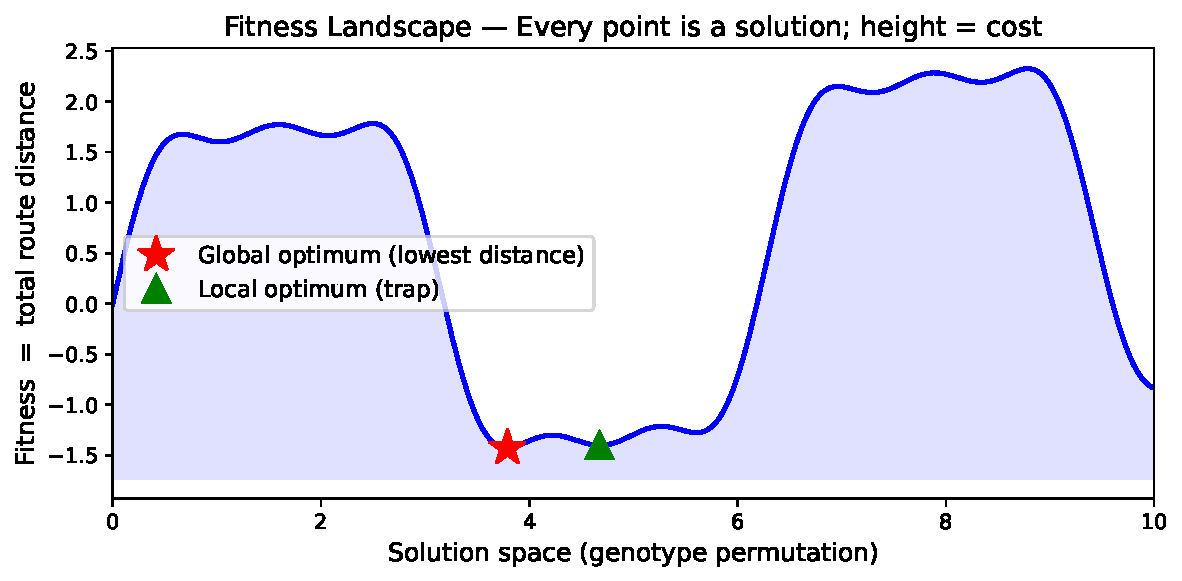
\includegraphics[width=0.72\linewidth]{fig_fitness_landscape.pdf}
  \end{center}

  The landscape is almost always \emph{multi-modal}: there are many local valleys (local optima)
  and a single deepest valley (the global optimum).
  A simple local search will fall into whichever valley it first encounters.
  An evolutionary algorithm maintains a \emph{population} of solutions spread across the landscape,
  allowing it to explore many valleys simultaneously and escape local optima through crossover and mutation.

  \framebreak

  \textbf{Why is this especially relevant to the CVRP?}
  The Capacitated Vehicle Routing Problem (CVRP) is NP-hard: exact methods become computationally
  infeasible for large instances.
  The search space grows factorially with the number of customers, so exhaustive enumeration is impossible.
  Evolutionary algorithms offer a practical alternative: they do not guarantee the global optimum,
  but they consistently find good solutions in reasonable time, and their flexibility means
  they can handle constraints such as vehicle capacity naturally through the solution representation.

  \begin{alertblock}{Key Insight}
    Evolutionary Algorithms do not require the objective function to be smooth, differentiable,
    or even well-defined mathematically — they only need to \emph{evaluate} a solution.
    This makes them extremely versatile for combinatorial problems like VRP.
  \end{alertblock}

\end{frame}

% ============================================================
\section{3.2 Evolutionary Algorithms}
% ============================================================

\begin{frame}[allowframebreaks]{3.2 Evolutionary Algorithms — Structure and Components}

  An Evolutionary Algorithm (EA) maintains a \textbf{population} of candidate solutions
  and improves them over many \emph{generations} (iterations) by applying biologically inspired operators.
  The book describes the specific variant used by the ACE Doughnuts case study,
  which follows the standard EA cycle shown below.

  \begin{center}
    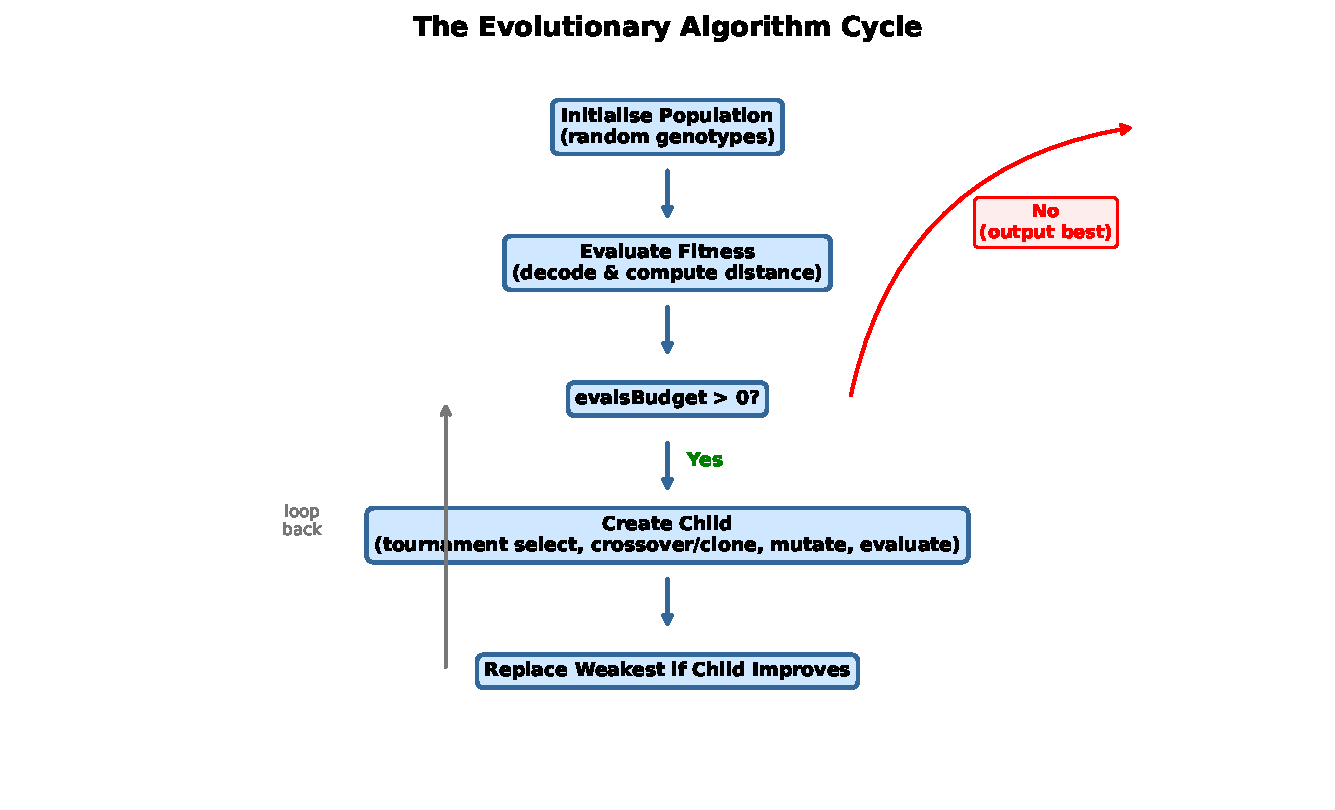
\includegraphics[width=0.65\linewidth]{fig_ea_cycle.pdf}
  \end{center}

  Each cycle generates one new child solution, evaluates it, and uses it to replace
  one of the weaker individuals in the population.
  This continues until a fixed \emph{evaluation budget} is exhausted.

  \framebreak

  \begin{block}{Algorithm 8: The Evolutionary Cycle (formal statement)}
    \textbf{Procedure} \texttt{EvolutionaryAlgorithm()}
    \begin{enumerate}
      \item Initialise a population of $N$ (N = population size) random solutions.
      \item Evaluate the fitness of every individual (compute total route distance).
      \item \textbf{While} the evaluation budget has not been exhausted:
        \begin{enumerate}
          \item Create a \emph{child} solution (see child creation procedure below).
          \item Select a \emph{weak} individual from the population via tournament selection.
          \item \textbf{If} the child is strictly better than the weak individual,
                replace the weak individual with the child.
          \item Track the best solution seen so far.
        \end{enumerate}
      \item \textbf{Return} the best solution found.
    \end{enumerate}
  \end{block}

  Note that the replacement step is \emph{conditional}: the child only enters the population
  if it improves on the individual it would replace.
  This ensures the average quality of the population never degrades, while still allowing
  new genetic material to enter if it is beneficial.

  \framebreak

  \textbf{The five components of an EA in detail:}

  \medskip
  \textbf{(1) Representation.}
  Before any evolution can happen, we must choose how to \emph{encode} a solution as a string of genes
  (the \emph{genotype}).
  For the CVRP, the book uses a \emph{grand-tour} encoding: the genotype is a single permutation
  of all customer IDs.
  The \emph{phenotype} (the actual vehicle routes) is \emph{decoded} from the genotype on demand
  by greedily splitting the tour wherever the vehicle capacity would be exceeded.
  We discuss this in detail in Section 3.3.

  \medskip
  \textbf{(2) Initialisation.}
  The initial population is created by generating $N$ random permutations of the customer list.
  Diversity is important here: a population of near-identical solutions will converge quickly
  to a local optimum, whereas a diverse population explores the search space more thoroughly.

  \medskip
  \textbf{(3) Fitness evaluation.}
  Each individual is scored by decoding its genotype into routes and summing the total travel
  distance.
  Lower distance means higher fitness (the problem is minimisation).

  \framebreak

  \textbf{(4) Selection — Tournament Selection.}
  To choose a parent for reproduction, the algorithm uses \emph{tournament selection}:
  draw $k$ (k = tournament size, usually 2) individuals at random from the population,
  and select the one with the \emph{lowest} fitness value (shortest distance).

  \begin{center}
    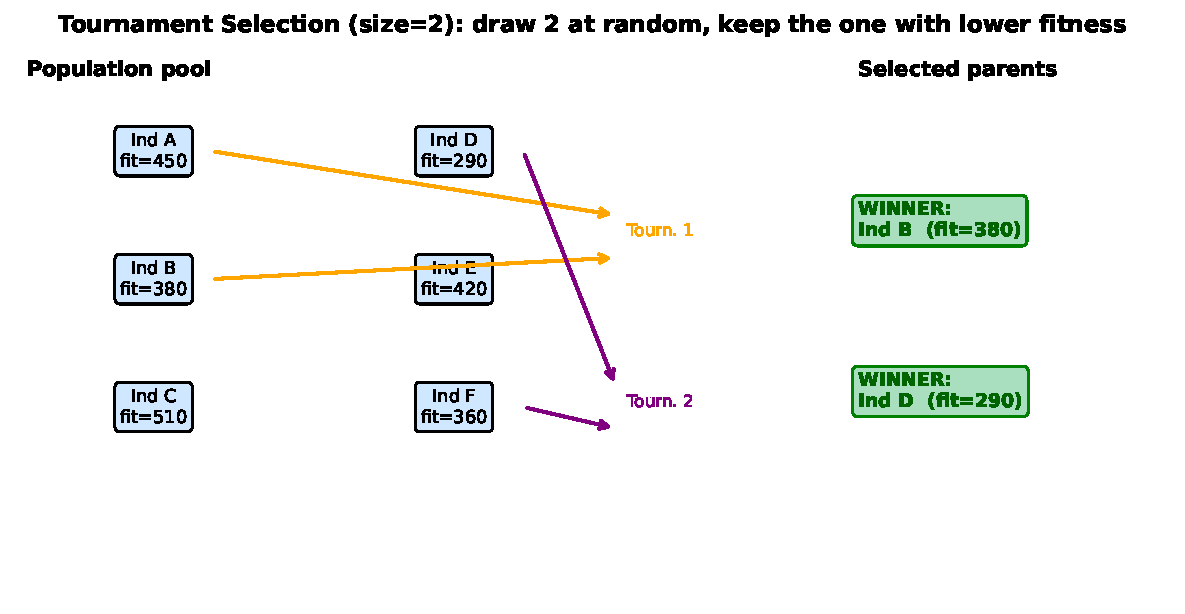
\includegraphics[width=0.72\linewidth]{fig_tournament_selection.pdf}
  \end{center}

  Tournament selection provides \emph{selection pressure}: better individuals are more likely
  to be chosen, but there is always a small chance that a worse individual is selected,
  which maintains diversity and prevents premature convergence.
  The parameter $k$ controls the pressure: larger $k$ means only the very best individuals
  are selected, reducing diversity; smaller $k$ means more randomness.

  \framebreak

  \textbf{(5) Replacement — Reverse Tournament Selection.}
  To decide \emph{which} member of the population to potentially replace,
  the algorithm runs a tournament in reverse: draw $k$ individuals at random and select
  the one with the \emph{highest} fitness (worst solution).
  If the new child is better than this worst individual, it replaces it;
  otherwise, the population is unchanged.
  This strategy removes weak individuals while preserving good ones.

  \begin{alertblock}{Key Insight: Steady-State vs.\ Generational EA}
    The book's EA is \emph{steady-state}: it replaces one individual per iteration.
    A \emph{generational} EA would replace the entire population each generation.
    Steady-state EAs update the population more smoothly and tend to preserve diversity better
    on a limited evaluation budget.
  \end{alertblock}

\end{frame}

% ============================================================
\section{3.3 Applying Evolution to the CVRP}
% ============================================================

\begin{frame}[allowframebreaks]{3.3 Applying Evolution to the CVRP — Representation}

  \textbf{The core challenge: how do we encode a VRP solution as a chromosome?}

  A VRP solution is a \emph{set of routes}, each starting and ending at the depot.
  Naively encoding routes directly creates problems for crossover:
  combining two valid route sets can produce duplicated or missing customers.
  The book solves this by using the \emph{grand-tour} representation.

  \medskip
  \begin{block}{Grand-Tour Representation}
    The \textbf{genotype} is a single permutation of all $n$ customer IDs,
    in the order they would be visited on a hypothetical single long tour.
    The \textbf{phenotype} (actual routes) is \emph{decoded} from the genotype by
    scanning through the list and starting a new route each time adding the next customer
    would cause the total demand to exceed the vehicle capacity $Q$ (Q = capacity limit).
  \end{block}

  \begin{center}
    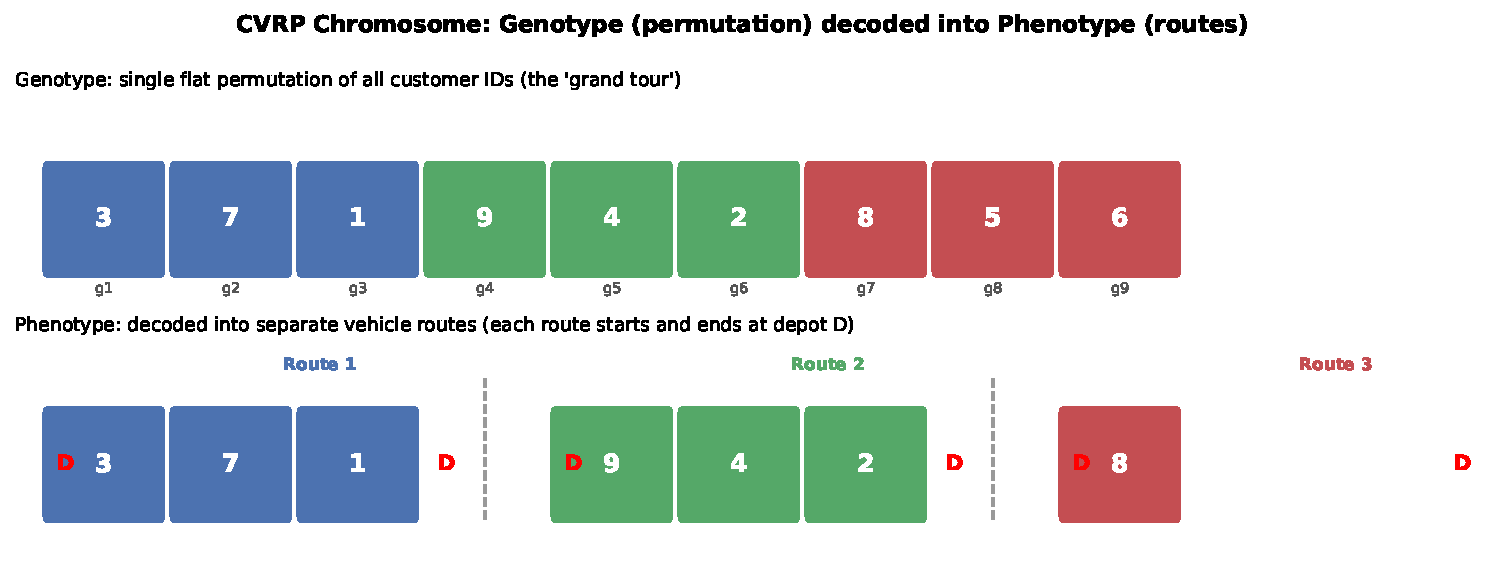
\includegraphics[width=0.85\linewidth]{fig_chromosome_encoding.pdf}
  \end{center}

  \framebreak

  \textbf{Worked example of decoding.}
  Suppose capacity $Q = 20$ and the genotype is $[3, 7, 1, 9, 4, 2, 8, 5, 6]$
  with demands $d_i$ (d subscript i = demand of customer $i$):
  $d_3=8,\ d_7=7,\ d_1=5,\ d_9=9,\ d_4=6,\ d_2=7,\ d_8=6,\ d_5=8,\ d_6=7$.

  \begin{exampleblock}{Worked Example: Decoding the Genotype}
    \begin{tabular}{lllll}
      \toprule
      Step & Customer & Demand & Route load so far & Action \\
      \midrule
      1 & 3 & 8  & 8  & add to Route 1 \\
      2 & 7 & 7  & 15 & add to Route 1 \\
      3 & 1 & 5  & 20 & add to Route 1 (exactly at limit) \\
      4 & 9 & 9  & 9  & 20+9 > 20, \textbf{start Route 2} \\
      5 & 4 & 6  & 15 & add to Route 2 \\
      6 & 2 & 7  & 22 & 15+7 > 20, \textbf{start Route 3} \\
      7 & 8 & 6  & 6  & add to Route 3 \\
      8 & 5 & 8  & 14 & add to Route 3 \\
      9 & 6 & 7  & 21 & 14+7 > 20, \textbf{start Route 4} \\
      \bottomrule
    \end{tabular}

    Result: Route 1 = D$\to$3$\to$7$\to$1$\to$D,  Route 2 = D$\to$9$\to$4$\to$D,
    Route 3 = D$\to$2$\to$8$\to$5$\to$D,  Route 4 = D$\to$6$\to$D.
  \end{exampleblock}

  The decoding always produces a \emph{feasible} solution (capacity never violated),
  because every genotype — even a random one — decodes to valid routes.
  This is an important property: the EA \emph{never} wastes evaluations on infeasible solutions.

  \framebreak

  \textbf{Genetic Operators — Crossover.}

  Crossover (also called \emph{recombination}) combines two parent genotypes to produce a child.
  For permutations, a simple two-point crossover would create duplicates, so the book uses
  \emph{Order-1 Crossover (OX)}:

  \medskip
  \begin{block}{Order-1 Crossover Procedure}
    Given two parent permutations P1 and P2:
    \begin{enumerate}
      \item Choose a random crossover point $x$ (a position in the chromosome).
      \item The child inherits genes $0, 1, \ldots, x-1$ directly from P1 (preserving order and position).
      \item The remaining genes are filled in from P2, scanning P2 left-to-right and adding each gene
            that has not yet appeared in the child.
    \end{enumerate}
    The result is a valid permutation containing every customer exactly once.
  \end{block}

  \begin{center}
    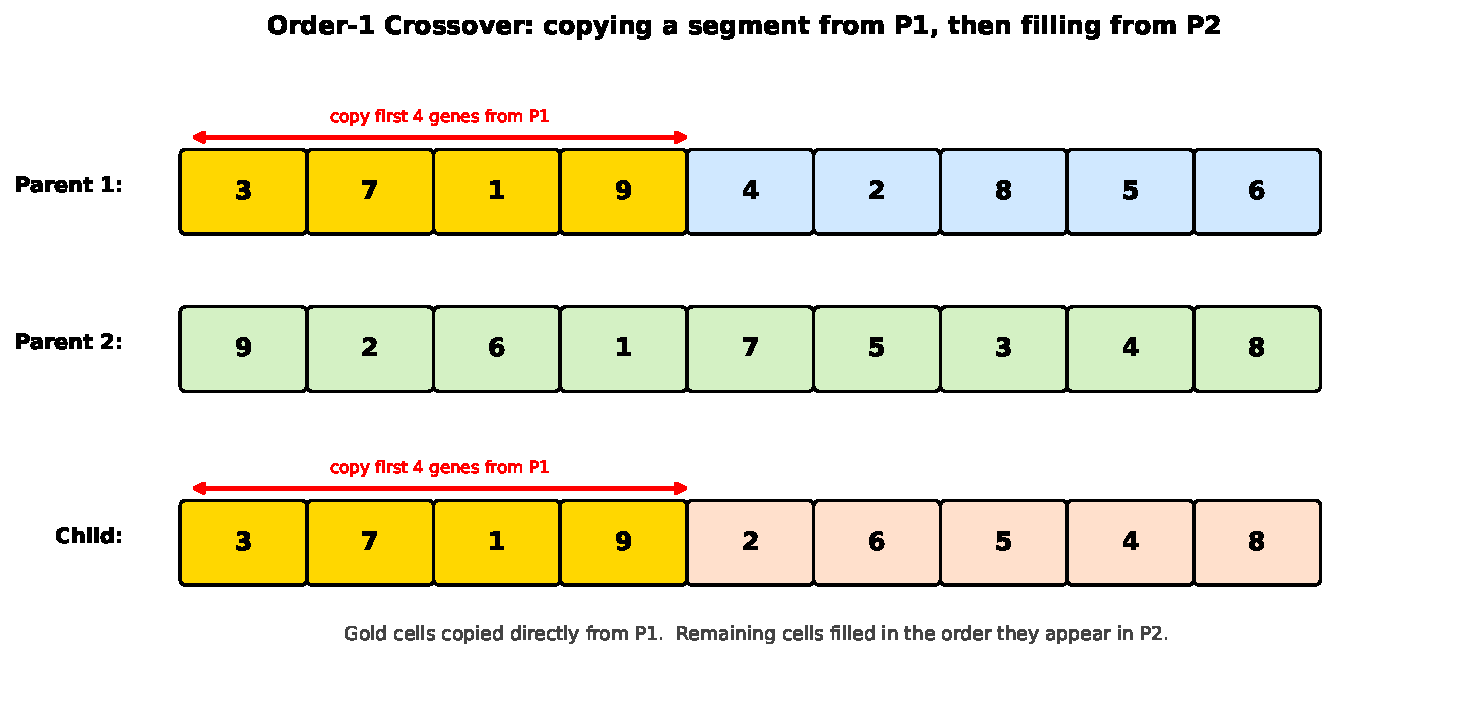
\includegraphics[width=0.82\linewidth]{fig_crossover.pdf}
  \end{center}

  \framebreak

  \textbf{Why does crossover help?}
  If P1 visits customers $\{3, 7, 1\}$ in a good sub-sequence (because they are geographically close),
  and P2 has a good sub-sequence for $\{9, 4, 2, 8\}$, the child may combine both good segments.
  This is the \emph{building block hypothesis}: short sequences of genes that work well together
  (called \emph{building blocks}) tend to be preserved and combined across generations.

  \begin{center}
    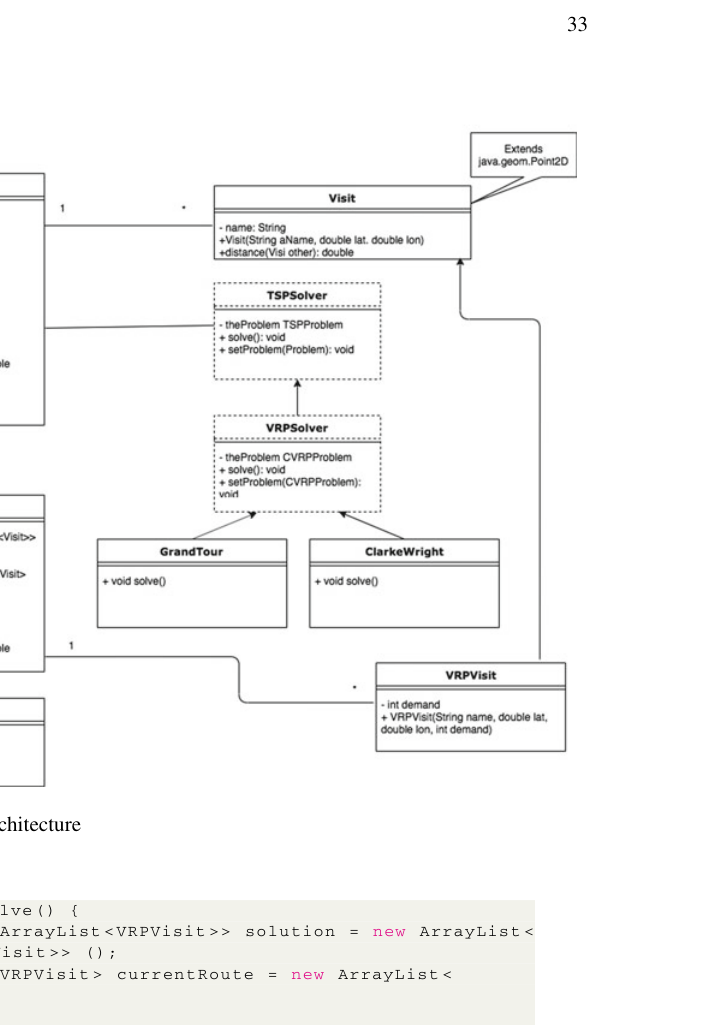
\includegraphics[width=0.62\linewidth]{fig_parent_child_routes.png}
  \end{center}

  The figure above (Fig.\ 3.1 from the book) shows two parent VRP solutions (phenotypes)
  and the child that results from their crossover.
  Notice how the child's routes inherit segments from both parents.

  \framebreak

  \textbf{Genetic Operators — Mutation.}

  Mutation introduces small random variations into a single individual's genotype.
  Without mutation, the EA can only recombine genes already present in the initial population;
  mutation allows entirely new gene values and orderings to appear, preventing stagnation.

  \medskip
  \begin{block}{Mutation Procedure (random relocation)}
    \begin{enumerate}
      \item Select a random gene (customer) from the genotype and \emph{remove} it.
      \item Choose a random insertion position in the remaining genotype.
      \item \emph{Insert} the gene at the new position.
    \end{enumerate}
    The genotype length stays the same; only the position of one customer changes.
  \end{block}

  \begin{center}
    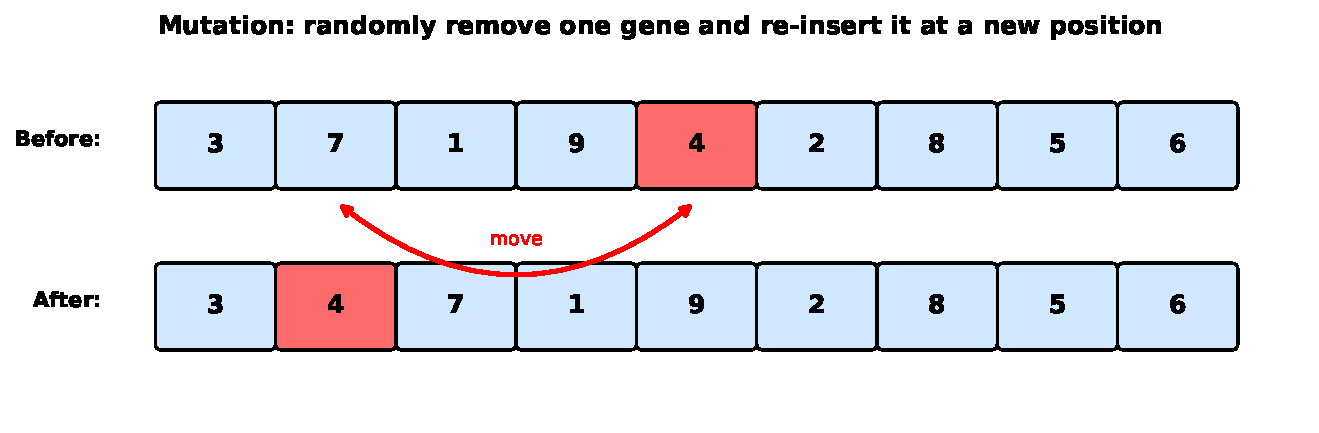
\includegraphics[width=0.78\linewidth]{fig_mutation.pdf}
  \end{center}

  In the example above, customer 4 is removed from position 4 and re-inserted at position 1.
  When the genotype is decoded, this customer will now be served in a different route
  and at a different point in the tour, potentially reducing the total distance.

\end{frame}

% ============================================================
\section{3.4 Choosing Parameters}
% ============================================================

\begin{frame}[allowframebreaks]{3.4 Choosing Parameters — Tuning the EA}

  \textbf{Evolutionary algorithms have several hyperparameters whose values significantly
  affect performance.}
  The book discusses the following parameters and their recommended values for the CVRP application.

  \medskip
  \begin{block}{Algorithm 9: Child Creation — Parameter Summary}
    \begin{tabular}{lll}
      \toprule
      \textbf{Parameter} & \textbf{Value used} & \textbf{Role} \\
      \midrule
      Population size        & 1{,}000    & Controls diversity of the search \\
      Evaluation budget      & 1{,}000{,}000 & Total number of fitness evaluations \\
      Crossover rate         & 0.5        & Probability of applying crossover \\
      Mutation rate          & 1.0        & Always apply mutation (to every child) \\
      Selection pressure     & tournament size 2 & Strength of parent selection \\
      Replacement pressure   & tournament size 2 & Strength of replacement selection \\
      \bottomrule
    \end{tabular}
  \end{block}

  The \emph{crossover rate} of 0.5 means that there is a 50\% chance the child is created
  by combining two parents; otherwise, the child is a copy (\emph{clone}) of a single parent.
  In both cases, mutation is always applied.
  A mutation rate of 1.0 means every child undergoes mutation — this is intentionally high
  to maintain diversity throughout the run.

  \framebreak

  \textbf{Child creation procedure in detail (Algorithm 9).}

  \begin{block}{Algorithm 9: CreateChild()}
    \begin{enumerate}
      \item With probability equal to the \emph{crossover rate}:
        \begin{enumerate}
          \item Select \emph{parent1} via tournament selection.
          \item Select \emph{parent2} via tournament selection.
          \item Create the child via \emph{crossover(parent1, parent2)}.
        \end{enumerate}
      \item Otherwise (no crossover):
        \begin{enumerate}
          \item Select a single \emph{parent} via tournament selection.
          \item The child is a \emph{copy} of that parent.
        \end{enumerate}
      \item Apply \emph{mutation} to the child.
      \item \emph{Evaluate} the child (decode genotype, compute total distance).
      \item \textbf{Return} child.
    \end{enumerate}
  \end{block}

  This two-path design allows the EA to exploit building blocks via crossover when it is
  productive, while still exploring via cloning-and-mutation when crossover would break
  good sub-sequences.

  \framebreak

  \textbf{Why is parameter choice hard?}

  Different problem instances may respond differently to the same parameter settings.
  A large population helps with diversity but means fewer generations are completed within
  a fixed evaluation budget.
  A high crossover rate can disrupt well-evolved sub-sequences; a very low rate loses the
  benefit of combining building blocks.

  \begin{center}
    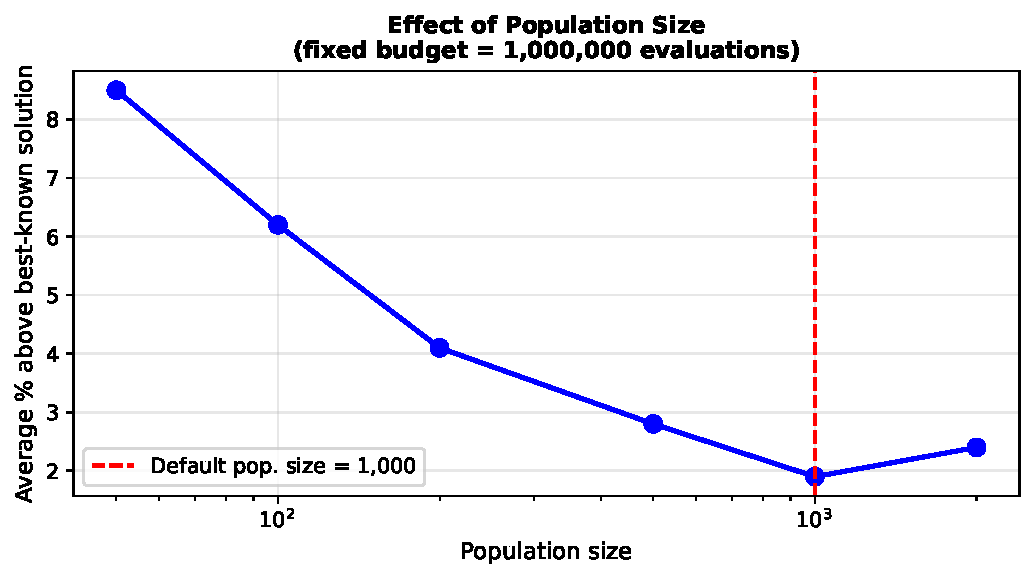
\includegraphics[width=0.60\linewidth]{fig_parameter_sensitivity.pdf}
  \end{center}

  The figure above illustrates a common pattern: solution quality improves as population
  size increases up to a point, then levels off or even worsens because each individual
  receives fewer evaluations within the budget.
  In practice, practitioners run the algorithm multiple times with different settings
  (parameter tuning) and select the configuration that performs best on average.
  The book cites Eiben and Smit (2012) as a reference on parameter tuning methods.

  \begin{alertblock}{Key Insight}
    There is no universally optimal parameter setting.
    The parameters recommended in this chapter (pop.\ size = 1{,}000; mutation rate = 1;
    crossover rate = 0.5) were chosen empirically for the Augerat CVRP benchmark instances
    and provide a reasonable starting point for similar problem sizes.
  \end{alertblock}

\end{frame}

% ============================================================
\section{3.5 Implementation}
% ============================================================

\begin{frame}[allowframebreaks]{3.5 Implementation — Architecture Overview}

  The book implements the EA in Java (the \emph{VRPea} class).
  This section explains the design, which can be straightforwardly translated to Python.

  \begin{center}
    
\includegraphics[width=0.72\linewidth]{fig_class_diagram.pdf}
  \end{center}

  The architecture has three main components:
  \begin{itemize}
    \item \textbf{VRPea} — the algorithm class, which contains the evolutionary cycle
          (Algorithm 8) and all selection/replacement logic.
    \item \textbf{Individual} — represents one candidate solution, holding both the
          genotype (the permutation) and the decoded phenotype (the routes).
          It also contains the \texttt{mutate()} and \texttt{evaluate()} methods.
    \item \textbf{CVRPProblem} — holds the problem instance data (customer demands,
          coordinates, vehicle capacity) and computes the total distance of a solution.
  \end{itemize}

  The separation between \texttt{Individual} and \texttt{CVRPProblem} is clean:
  the individual owns the solution representation; the problem owns the data.
  This design makes it easy to swap out the problem type or the representation
  without rewriting the evolutionary loop.

  \framebreak

  \textbf{The Individual class — genotype and phenotype.}

  The genotype is stored as an \texttt{ArrayList<VRPVisit>} (a list of customer visit objects).
  The phenotype is stored as an \texttt{ArrayList<ArrayList<VRPVisit>>} (a list of routes,
  each route being a list of visits).
  Crucially, the phenotype is \textbf{lazy}: it is set to \texttt{null} initially and only
  computed when \texttt{evaluate()} is called.
  If the genotype is later mutated, the phenotype is invalidated (set back to \texttt{null})
  so it will be recomputed on the next evaluation.

\end{frame}

\begin{frame}[fragile]{3.5 Java: The Main Evolutionary Loop (Listing 3.1)}

  The following Java code is the core of the \texttt{VRPea.solve()} method.
  It implements Algorithm 8 exactly as described above.

  \begin{lstlisting}[style=javastyle,caption={Listing 3.1 -- The evolutionary algorithm (VRPea.solve())}]
private RandomSingleton rnd = RandomSingleton.getInstance();
private int POP_SIZE = 500;
private int TOUR_SIZE = 2;
private double XO_RATE = 0.7;
private int evalsBudget = 1000000;

@Override
public void solve() {
    // Reference to the best individual in the population
    Individual bestSoFar = InitialisePopution();
    while (evalsBudget > 0) {
        // Create child
        Individual child = null;
        if (rnd.getRnd().nextDouble() < XO_RATE) {
            // Create a new Individual using recombination,
            // randomly selecting the parents
            child = new Individual(super.theProblem,
                tournamentSelection(TOUR_SIZE),
                tournamentSelection(TOUR_SIZE));
        } else {
            // Create a child by copying a single parent
            child = tournamentSelection(TOUR_SIZE).copy();
        }
        child.mutate();
        child.evaluate();
        evalsBudget--;
        // Select an Individual with a poor fitness to be replaced
        Individual poor = tournamentSelectWorst(TOUR_SIZE);
        if (poor.evaluate() > child.evaluate()) {
            // Only replace if the child is an improvement
            if (child.evaluate() < bestSoFar.evaluate()) {
                bestSoFar = child;
            }
            population.remove(poor);
            population.add(child);
        }
    }
    super.theProblem.setSolution(bestSoFar.getPhenotype());
}
  \end{lstlisting}

\end{frame}

\begin{frame}[fragile]{3.5 Java: Genotype/Phenotype and Constructors (Listings 3.2 \& 3.3)}

  \begin{lstlisting}[style=javastyle,caption={Listing 3.2 -- Genotype and phenotype fields within Individual}]
// The genotype is a "grand tour" list of visits
private ArrayList<VRPVisit> genotype;
// The phenotype is a set of routes created from the genotype
private ArrayList<ArrayList<VRPVisit>> phenotype;
  \end{lstlisting}

  \medskip

  \begin{lstlisting}[style=javastyle,caption={Listing 3.3 -- Constructors for Individual}]
public Individual(CVRPProblem prob) {
    // Constructor to create a new random genotype
    problem = prob;
    genotype = new ArrayList<VRPVisit>();
    for (Visit v : prob.getSolution()) {
        genotype.add((VRPVisit)v);
    }
    genotype = randomize(genotype);
    phenotype = null;
}
public Individual(CVRPProblem prob, Individual parent1, Individual parent2) {
    // Create a new Individual via recombination of parent1 and parent2
    problem = prob;
    genotype = new ArrayList<VRPVisit>();
    int xPoint = rnd.getRnd().nextInt(parent1.genotype.size());
    for (int count = 0; count < xPoint; count++) {
        genotype.add(parent1.genotype.get(count)); // copy p1[0..xPoint)
    }
    for (int count = 0; count < parent2.genotype.size(); count++) {
        VRPVisit v = parent2.genotype.get(count);
        if (!genotype.contains(v)) { genotype.add(v); } // fill from p2
    }
}
  \end{lstlisting}

\end{frame}

\begin{frame}[fragile]{3.5 Java: Mutation and Evaluate (Listings 3.4 \& 3.5)}

  \textbf{Mutation} (Listing 3.4) randomly removes one gene and re-inserts it at a new position.
  Notice that the phenotype is immediately invalidated (set to \texttt{null}) after mutation,
  so the outdated route set is never accidentally used.

  \begin{lstlisting}[style=javastyle,caption={Listing 3.4 -- Individual.mutate()}]
public void mutate() {
    // Mutate the genotype by randomly moving a gene.
    phenotype = null;
    int rndGene = rnd.getRnd().nextInt(genotype.size());
    VRPVisit v = genotype.remove(rndGene);
    int addPoint = rnd.getRnd().nextInt(genotype.size());
    genotype.add(addPoint, v);
}
  \end{lstlisting}

  \textbf{Evaluate} (Listing 3.5) lazily builds the phenotype, then calls the problem's
  \texttt{getDistance()} method.
  It scans the genotype left-to-right; each time the next customer would cause the route's
  total demand to exceed the capacity, a new route is started.

  \begin{lstlisting}[style=javastyle,caption={Listing 3.5 -- Individual.evaluate()}]
public double evaluate() {
    if (phenotype == null) {
        phenotype = new ArrayList<ArrayList<VRPVisit>>();
        ArrayList<VRPVisit> newRoute = new ArrayList<VRPVisit>();
        for (VRPVisit v : genotype) {
            if (v.getDemand() + routeDemand(newRoute) > problem.getCapacity()) {
                phenotype.add(newRoute);   // capacity exceeded: start new route
                newRoute = new ArrayList<VRPVisit>();
            }
            newRoute.add(v);
        }
        phenotype.add(newRoute);
    }
    return problem.getDistance(phenotype);
}
  \end{lstlisting}

\end{frame}

\begin{frame}[fragile]{3.5 Python Translation — Core EA Loop}

  The following Python code faithfully translates the Java EA into idiomatic Python.
  Understanding the Python version is useful for experimentation, as it is more accessible
  than the Java original.

  \begin{lstlisting}[style=pythonstyle,caption={Python: main evolutionary loop}]
import random
import copy

class VRPea:
    def __init__(self, problem, pop_size=500, tour_size=2,
                 xo_rate=0.7, evals_budget=1_000_000):
        self.problem = problem    # CVRPProblem instance
        self.POP_SIZE = pop_size  # number of individuals in population
        self.TOUR_SIZE = tour_size  # tournament size for selection
        self.XO_RATE = xo_rate    # crossover probability
        self.evals_budget = evals_budget  # total evaluation count

    def solve(self):
        population = self._initialise_population()
        best = min(population, key=lambda ind: ind.evaluate())

        while self.evals_budget > 0:
            if random.random() < self.XO_RATE:
                # Crossover: select two parents, combine them
                p1 = self._tournament_select(population)
                p2 = self._tournament_select(population)
                child = Individual(self.problem, p1, p2)
            else:
                # Clone: copy one parent
                p = self._tournament_select(population)
                child = copy.deepcopy(p)

            child.mutate()
            child.evaluate()
            self.evals_budget -= 1

            # Replace worst individual if child is better
            poor = self._tournament_select_worst(population)
            if child.fitness < poor.fitness:
                population.remove(poor)
                population.append(child)
                if child.fitness < best.fitness:
                    best = child

        return best.phenotype
  \end{lstlisting}

\end{frame}

\begin{frame}[fragile]{3.5 Python Translation — Individual Class}

  \begin{lstlisting}[style=pythonstyle,caption={Python: Individual class with genotype/phenotype}]
class Individual:
    def __init__(self, problem, parent1=None, parent2=None):
        self.problem = problem
        self.phenotype = None  # lazily computed
        self.fitness = None

        if parent1 is None:
            # Random initialisation
            self.genotype = list(problem.customers)
            random.shuffle(self.genotype)
        else:
            # Order-1 crossover of two parents
            xp = random.randint(0, len(parent1.genotype))
            self.genotype = list(parent1.genotype[:xp])
            for gene in parent2.genotype:
                if gene not in self.genotype:
                    self.genotype.append(gene)

    def mutate(self):
        """Remove one random gene and re-insert it at a new position."""
        self.phenotype = None  # invalidate cached phenotype
        self.fitness = None
        idx = random.randint(0, len(self.genotype) - 1)
        gene = self.genotype.pop(idx)
        new_pos = random.randint(0, len(self.genotype))
        self.genotype.insert(new_pos, gene)

    def evaluate(self):
        """Decode genotype to routes, then compute total distance."""
        if self.fitness is None:
            self.phenotype = self._decode()
            self.fitness = self.problem.total_distance(self.phenotype)
        return self.fitness

    def _decode(self):
        """Split grand tour into routes wherever capacity would be exceeded."""
        routes, route, load = [], [], 0
        for customer in self.genotype:
            demand = self.problem.demand[customer]
            if load + demand > self.problem.capacity:
                routes.append(route)  # start a new route
                route, load = [], 0
            route.append(customer)
            load += demand
        if route:
            routes.append(route)
        return routes
  \end{lstlisting}

\end{frame}

\begin{frame}[fragile]{3.5 Python Translation — Selection and Hybrid Solver}

  \begin{lstlisting}[style=pythonstyle,caption={Python: tournament selection and hybrid solver}]
def _tournament_select(self, population):
    """Return the individual with the lowest fitness from a random sample."""
    sample = random.sample(population, self.TOUR_SIZE)
    return min(sample, key=lambda ind: ind.evaluate())

def _tournament_select_worst(self, population):
    """Return the individual with the highest fitness from a random sample."""
    sample = random.sample(population, self.TOUR_SIZE)
    return max(sample, key=lambda ind: ind.evaluate())

def _initialise_population(self):
    """Create POP_SIZE random individuals and evaluate them all."""
    pop = [Individual(self.problem) for _ in range(self.POP_SIZE)]
    for ind in pop:
        ind.evaluate()
    return pop


# -- Hybrid solver: run Clarke-Wright first, then refine with EA --
def hybrid_solve(problem, n_ea_runs=20):
    """
    Run Clarke-Wright to get a warm start, then run the EA 20 times
    (because the EA is stochastic) and report the best result found.
    """
    cw = ClarkeWright(problem)
    cw_solution = cw.solve()
    cw_distance = problem.total_distance(cw_solution)

    best_ea_distance = float('inf')
    best_ea_solution = None

    for seed in range(n_ea_runs):
        random.seed(seed)
        ea = VRPea(problem)
        solution = ea.solve()
        dist = problem.total_distance(solution)
        if dist < best_ea_distance:
            best_ea_distance = dist
            best_ea_solution = solution

    print(f"Clarke-Wright distance: {cw_distance:.2f}")
    print(f"EA best distance (20 runs): {best_ea_distance:.2f}")
    return best_ea_solution
  \end{lstlisting}

  The hybrid approach (Listing 3.6 in the book) runs the EA 20 times with different random seeds
  and keeps the best result.
  Because the EA is \emph{stochastic} (random), it can produce a different result on each run;
  running it multiple times significantly reduces the risk of returning a poor solution.

\end{frame}

% ============================================================
\section{3.6 Results}
% ============================================================

\begin{frame}[allowframebreaks]{3.6 Results — Benchmarking on Augerat Instances}

  ACE Doughnuts test the EA on the \textbf{Augerat (1995) benchmark} instances —
  a well-known collection of CVRP test problems from the literature.
  The instances are grouped into three sets:
  \textbf{Set A} (31--80 customers),
  \textbf{Set B} (31--78 customers),
  and \textbf{Set P} (16--101 customers).
  For each instance, the optimal (or best-known) solution from exact branch-and-cut methods
  is available, allowing a direct comparison.

  \medskip
  Because the EA is stochastic, it is run \textbf{20 times} per instance.
  The reported result is the \emph{best} solution found across the 20 runs.

  \begin{alertblock}{Interpretation Caveat}
    The EA rarely finds the provably optimal solution (that would require an exact solver),
    but it consistently finds solutions close to optimal in far less time.
    The question is how large the gap is.
  \end{alertblock}

  \framebreak

  \textbf{Results on Set A (Table 3.1 excerpt).}

  \begin{center}
    \small
    \begin{tabular}{lccccc}
      \toprule
      Problem & $n$ & B\&C best & EA distance & Vehicles & \% over B\&C \\
      \midrule
      A-n32-k5  & 31 & 784  & 797.9  & 5 & 1.77\% \\
      A-n33-k5  & 32 & 661  & 662.1  & 5 & 0.17\% \\
      A-n33-k6  & 32 & 742  & 742.7  & 6 & 0.09\% \\
      A-n34-k5  & 33 & 778  & 786.4  & 5 & 1.08\% \\
      A-n36-k5  & 35 & 799  & 810.1  & 5 & 1.39\% \\
      A-n37-k5  & 36 & 669  & 682.3  & 5 & 1.99\% \\
      A-n38-k5  & 37 & 730  & 736.5  & 5 & 0.90\% \\
      A-n39-k5  & 38 & 822  & 845.1  & 5 & 2.81\% \\
      A-n44-k7  & 43 & 937  & 978.6  & 6 & 4.44\% \\
      A-n45-k6  & 44 & 944  & 963.7  & 6 & 2.05\% \\
      \bottomrule
    \end{tabular}
  \end{center}

  The symbol $n$ denotes the number of customers (excluding the depot).
  ``B\&C best'' is the best solution found by branch-and-cut (Augerat 1995).
  ``\% over B\&C'' is the percentage by which the EA's best result exceeds the B\&C result.
  On smaller instances (e.g.\ A-n33-k5, A-n33-k6), the EA comes within 0.1--0.2\%
  of the optimal solution.

  \framebreak

  \textbf{Results on Set B (Table 3.2 excerpt).}

  \begin{center}
    \small
    \begin{tabular}{lccccc}
      \toprule
      Problem & $n$ & B\&C best & EA distance & Vehicles & \% over B\&C \\
      \midrule
      B-n31-k5  & 31 & 672 & 676.1 & 5 & 0.61\% \\
      B-n34-k5  & 34 & 788 & 790.9 & 5 & 0.36\% \\
      B-n38-k6  & 38 & 805 & 809.7 & 6 & 0.58\% \\
      B-n39-k5  & 39 & 549 & 564.7 & 5 & 2.86\% \\
      B-n41-k6  & 41 & 829 & 839.7 & 6 & 1.29\% \\
      B-n43-k6  & 43 & 742 & 758.1 & 6 & 2.17\% \\
      B-n44-k7  & 44 & 909 & 947.3 & 7 & 4.22\% \\
      B-n50-k8  & 50 & 1313 & 1342.0 & 8 & 2.21\% \\
      B-n52-k7  & 52 & 747 & 778.2 & 7 & 4.17\% \\
      B-n57-k9  & 57 & 1598 & 1668.6 & 9 & 4.42\% \\
      \bottomrule
    \end{tabular}
  \end{center}

  Set B results are similar in character to Set A: on smaller instances the gap is very small,
  while on larger, harder instances (more customers, more vehicles) the gap grows somewhat.
  The EA \emph{always} finds the same number of vehicles as the B\&C solution,
  indicating that the route structure is correct even when the exact distances differ slightly.

  \framebreak

  \textbf{Results on Set P (Table 3.3 excerpt) — includes larger instances.}

  \begin{center}
    \small
    \begin{tabular}{lccccc}
      \toprule
      Problem & $n$ & B\&C best & EA distance & Vehicles & \% over B\&C \\
      \midrule
      P-n16-k8  & 16  & 435  & 451.3  & 8  & 3.76\% \\
      P-n19-k2  & 19  & 212  & 212.7  & 2  & 0.31\% \\
      P-n20-k2  & 20  & 220  & 217.4  & 2  & $-1.17\%$ \\
      P-n22-k2  & 22  & 216  & 217.9  & 2  & 0.86\% \\
      P-n40-k5  & 40  & 458  & 464.7  & 5  & 1.46\% \\
      P-n45-k5  & 45  & 510  & 535.7  & 5  & 5.04\% \\
      P-n55-k7  & 55  & 524  & 586.2  & 7  & 11.87\% \\
      P-n60-k10 & 60  & 856  & 996.4  & 16 & 16.40\% \\
      P-n70-k10 & 70  & 834  & 942.4  & 10 & 13.00\% \\
      P-n101-k4 & 101 & 681  & 929.9  & 4  & 36.56\% \\
      \bottomrule
    \end{tabular}
  \end{center}

  Three remarkable observations:
  (1) On P-n20-k2, the EA actually finds a \emph{shorter} route than the branch-and-cut result
  ($-1.17\%$), likely due to rounding differences between software platforms.
  (2) On very large instances (P-n101-k4, 101 customers), the gap widens considerably (36.56\%).
  (3) On some large instances, the EA uses more vehicles than the B\&C solution.

  \framebreak

  \textbf{EA versus Clarke-Wright: who finds the best solution? (Table 3.4 summary)}

  \begin{center}
    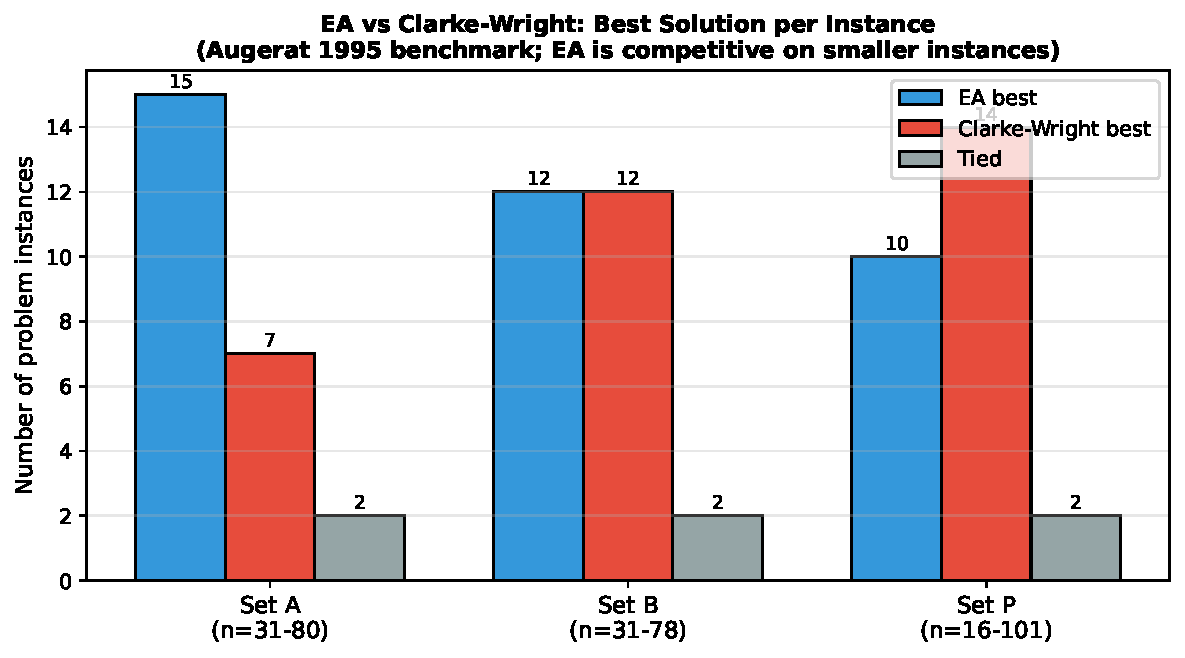
\includegraphics[width=0.78\linewidth]{fig_ea_vs_cw.pdf}
  \end{center}

  The figure above summarises the Table 3.4 comparison.
  The EA tends to win on smaller instances (Set A), where population-based search can
  effectively explore the space within the budget.
  Clarke-Wright becomes more competitive on larger instances (Set P), which is not surprising:
  Clarke-Wright is a deterministic greedy heuristic that scales well,
  while the EA's population diversity advantage diminishes when each individual represents a
  complex large tour.

  \framebreak

  \textbf{The convergence behaviour of the EA.}

  \begin{center}
    
\includegraphics[width=0.82\linewidth]{fig_convergence.pdf}
  \end{center}

  The left plot shows a typical EA run: the fitness (total distance) drops rapidly in the
  first few minutes as the population quickly improves, then slows down as the algorithm
  approaches a local optimum.
  This is the characteristic \emph{convergence} behaviour of EAs.

  The right plot introduces two user-defined thresholds:
  $Q$ (Q = quality threshold) is the maximum distance the user will accept,
  and $T$ (T = patience threshold, in seconds) is the maximum time the user is willing to wait.
  A solution is considered \emph{acceptable} if the fitness drops below $Q$ before time $T$.
  The shaded region is the ``acceptable zone'': if the convergence curve enters this zone,
  the algorithm has found a satisfactory solution in time.

\end{frame}

% ============================================================
\section{3.7 Conclusions}
% ============================================================

\begin{frame}[allowframebreaks]{3.7 Conclusions}

  \textbf{What has been achieved in this chapter?}

  The chapter demonstrated how a biologically-inspired Evolutionary Algorithm can be applied
  to the Capacitated Vehicle Routing Problem.
  Starting from the analogy of natural selection, the chapter built a complete, working EA
  for the CVRP, covering representation, operators, selection, and parameter choice.

  \medskip
  \begin{block}{Summary of the EA approach}
    \begin{itemize}
      \item The \emph{grand-tour genotype} encodes any CVRP solution as a simple
            permutation of customer IDs, guaranteeing feasibility after decoding.
      \item \emph{Order-1 crossover} combines building blocks from two parents
            while preserving the constraint that each customer appears exactly once.
      \item \emph{Random relocation mutation} keeps the search exploring and prevents
            the population from converging prematurely.
      \item \emph{Tournament selection} (for both parents and replacement) provides
            tunable selection pressure without requiring fitness scaling.
    \end{itemize}
  \end{block}

  \framebreak

  \textbf{Key findings from the benchmarks.}

  \begin{itemize}
    \item On smaller instances (31--50 customers), the EA finds solutions within 1--3\%
          of the branch-and-cut optimum, which is excellent for a metaheuristic.
    \item The EA consistently uses the same number of vehicles as the optimal solution,
          meaning it finds the correct routing structure even if individual routes are not
          perfectly optimised.
    \item On larger instances (60--101 customers), the gap grows — the EA still finds
          good solutions, but they are further from optimal.
    \item Neither the EA nor Clarke-Wright dominates the other across all instances:
          the best strategy depends on the specific instance size and structure.
  \end{itemize}

  \textbf{Practical recommendation for ACE Doughnuts:}
  Run both Clarke-Wright and the EA (multiple times), then take the best result.
  The book's Algorithm 3.6 (the hybrid solver) does exactly this.
  This portfolio approach hedges against the weaknesses of each individual method.

  \framebreak

  \textbf{Limitations and open questions.}

  \begin{enumerate}
    \item \textbf{Stochasticity} — Because the EA is random, it can produce a different result
          each run.
          Running it 20 times mitigates this but adds computational cost.
          A real deployment would need to balance solution quality against available time.
    \item \textbf{Parameter sensitivity} — The parameters (population size, crossover rate, etc.)
          were tuned for the Augerat instances.
          They may need re-tuning for significantly different problem sizes or structures.
    \item \textbf{Large instance scalability} — The 36\% gap on P-n101 shows that the
          basic EA does not scale as well as heuristics for very large instances.
          More sophisticated operators (e.g.\ local search within the EA, also known as
          a \emph{memetic algorithm}) could close this gap.
    \item \textbf{Single objective} — This chapter optimised total distance only.
          Real-world delivery problems often have multiple objectives (time windows, driver costs,
          CO\textsubscript{2} emissions), which are addressed in later chapters.
  \end{enumerate}

  \begin{alertblock}{Chapter Takeaway}
    Evolutionary Algorithms offer a flexible, powerful approach to the CVRP.
    They require no problem-specific mathematical analysis, scale to real-world instance sizes,
    and can be adapted to new constraints by modifying only the representation and evaluation function.
    Their main cost is the need for many fitness evaluations and careful parameter selection.
  \end{alertblock}

  \framebreak

  \textbf{References cited in this chapter.}

  \begin{itemize}
    \item Augerat, P.\ (1995). \emph{Approche poly\`edrale du probl\`eme de tourn\'ees de
          v\'ehicules.} PhD Thesis, Grenoble Institute of Technology.
    \item Augerat, P.\ (2014a/b/c). VRP-REP benchmark datasets (Sets A, B, P).
    \item Darwin, C.\ (1859). \emph{On the Origin of Species by Means of Natural Selection.}
          John Murray, London.
    \item Eiben, A.E.\ \& Smit, S.K.\ (2012). Evolutionary Algorithm Parameters and Methods
          to Tune Them. In \emph{Autonomous Search}, Springer.
    \item Goldberg, D.\ (1989). \emph{Genetic Algorithms in Search, Optimization and
          Machine Learning.} Addison-Wesley.
    \item Holland, J.H.\ (1975). \emph{Adaptation in Natural and Artificial Systems.}
          University of Michigan Press.
  \end{itemize}

\end{frame}

% ── summary frame ─────────────────────────────────────────────
\begin{frame}{Chapter 3 — One-Slide Summary}

  \begin{columns}
    \column{0.52\textwidth}
    \begin{block}{What is an Evolutionary Algorithm?}
      A population-based search method inspired by natural selection.
      It maintains $N$ candidate solutions and iteratively creates children
      via crossover and mutation, replacing weak individuals when children improve on them.
    \end{block}
    \vspace{0.5em}
    \begin{block}{CVRP Representation}
      \textbf{Genotype}: permutation of customer IDs (grand tour).\\
      \textbf{Phenotype}: routes decoded by splitting at capacity limits.\\
      Any permutation decodes to a \emph{feasible} solution.
    \end{block}
    \vspace{0.5em}
    \begin{alertblock}{Bottom Line}
      EA finds solutions within 1--5\% of optimal on medium instances
      in practical time.  Combine with Clarke-Wright for best real-world results.
    \end{alertblock}

    \column{0.46\textwidth}
    \begin{block}{Key Parameters}
      \begin{tabular}{ll}
        Population size    & 1{,}000 \\
        Evaluation budget  & 1{,}000{,}000 \\
        Crossover rate     & 0.5 \\
        Mutation rate      & 1.0 (always) \\
        Tournament size    & 2 \\
      \end{tabular}
    \end{block}
    \vspace{0.5em}
    \begin{block}{Operators}
      \textbf{Selection}: tournament (draw 2, keep best).\\
      \textbf{Crossover}: Order-1 (copy prefix from P1, fill from P2).\\
      \textbf{Mutation}: remove one gene, re-insert at random position.\\
      \textbf{Replacement}: reverse tournament (remove worst).
    \end{block}
  \end{columns}

\end{frame}

\end{document}
